\documentclass[12pt,a4paper]{article}
\usepackage[T2A]{fontenc}
\usepackage[utf8]{inputenc}
\usepackage[russian]{babel}
\usepackage{amsmath}
\usepackage{amssymb}
\usepackage{graphicx}
\usepackage{floatrow}

\newcommand{\figref}[1]{(См. рис. \ref{#1})}
\newcommand{\secref}[1]{(См. раздел. \ref{#1})}

\newcommand{\e}[1]{\text{$\cdot10^{#1}$}}



\author{\normalsize Выполнил: Дедков Денис, группа Б01-109 \\
	\normalsize 14.02.2022}
\date{}



\usepackage{float}
\restylefloat{table}
\title{
	\large Отчет о выполнении лабораторной работы 2.1.6 \\
	\Large Эффект Джоуля-Томсона \\ 
	
}


\begin{document}
	\maketitle
	\subsection*{Цель работы} 
	 Определение изменения температуры углекислого газа при протекании через малопроницаемую перегородку при разных начальных значениях давления и температуры;
	 вычисление по результатам опытов коэффициентов Ван-дер-Ваальса $a$ и $b$.
	
	\subsection*{Оборудование и приборы} Трубка с пористой перегородкой; труба Дьюара; термостат; термометры; дифференциальная термопара; микровольтметр; балластный баллон; манометр.
	
\subsection*{Теоретическое введение}
Эффектом Джоуля–Томсона называется изменение температуры газа, медленно протекающего из области высокого в область низкого давления в условиях хорошей тепловой изоляции. В разреженных газах, которые приближаются по своим свойствам к идеальному газу, при таком течении температура газа не меняется. Эффект Джоуля–Томсона демонстрирует отличие исследуемого газа от идеального.

В работе исследуется изменение температуры углекислого газа при медленном его течении по трубке с пористой перегородкой (риc. \ref{ust}). Трубка 1 хорошо теплоизолирована. Величина эффекта Джоуля–Томсона определяется по разности температуры газа до и после перегородки.

Рассмотрим стационарный поток газа между произвольными сечениями I и II трубки. Пусть, для определенности, через трубку прошел 1 моль углекислого газа; $ \mu $ -- его молярная масса. Молярные объемы газа, его давления и отнесенные к молю внутренние энергии газа в сечениях I и II обозначим соответственно $ V_1, P_1, U_1 $ и $ V_2, P_2, U_2 $. Для того чтобы ввести в трубку объем $ V_1 $, над газом нужно совершить работу $ A_1 = P_1V_1 $. Проходя через сечение II, газ сам совершает работу $ A_2 = P_2V_2 $. Так как через боковые стенки не происходит ни обмена теплом, ни передачи механической энергии, то

\begin{equation}\label{1}
	A_1-A_2=\left(U_2+\frac{\mu v_2^2}{2}\right) - \left(U_1 + \frac{\mu v_1^2}{2}\right).
\end{equation}

В уравнении \eqref{1} учтено изменение как внутренней (первые члены в скобках), так и кинетической (вторые члены в скобках) энергии газа. Подставляя в \eqref{1} написанные выражения для $ A_1 $ и $ A_2 $ и перегруппировывая члены, найдем

\begin{equation}\label{2}
	H_1-H_2=\left(U_1+P_1V_1\right) - \left(U_2 + P_2V_2\right) = \frac{1}{2} \mu \left(v^2_2-v^2_1\right).
\end{equation}

Сделаем несколько замечаний. Прежде всего отметим, что в процессе Джоуля–Томсона газ испытывает в пористой перегородке существенное трение, приводящее к ее нагреву. Потери энергии на нагрев трубки в начале процесса могут быть очень существенными и сильно искажают ход явления. После того как температура трубки установится и газ станет уносить с собой все выделенное им в пробке тепло, формула \eqref{1} становится точной, если, конечно, теплоизоляция трубки достаточно хороша и не происходит утечек тепла наружу через ее стенки.

Второе замечание связано с правой частью \eqref{2}. Процесс Джоуля–Томсона в чистом виде осуществляется лишь в том случае, если правой частью можно пренебречь, т. е. если макроскопическая скорость газа с обеих сторон трубки достаточно мала. У нас сейчас нет критерия, который позволил бы установить, когда это можно сделать. В силу сохранения энтропии в случае реального газа получаем:

\begin{equation}\label{3}
	\mu_\text{Д--Т} = \frac{\Delta T}{\Delta P} \approx \frac{\frac{2a}{T} - b}{C_P}.
\end{equation}

Из формулы \eqref{3} видно, что эффект Джоуля–Томсона для не очень плотного газа зависит от соотношения величин $ a $ и $ b $, которые оказывают противоположное влияние на знак эффекта. Если силы взаимодействия между молекулами велики, так что превалирует <<поправка на давление>>, то основную роль играет член, содержащий $a$, и 

$$ \frac{\Delta T}{\Delta P} > 0, $$
т. е. газ при расширении охлаждается ($ \Delta T < 0 $, так как всегда $ \Delta P < 0 $). В обратном случае (малые $ a $)

$$ \frac{\Delta T}{\Delta P} < 0, $$
т. е. газ нагревается ($ \Delta T > 0 $, так как по-прежнему $ \Delta P < 0 $).

Этот результат нетрудно понять из энергетических соображений. Как мы уже знаем, у идеального газа эффект Джоуля–Томсона отсутствует. Идеальный газ отличается от реального тем, что в нем можно пренебречь потенциальной энергией взаимодействия молекул. Наличие этой энергии приводит к охлаждению или нагреванию реальных газов при расширении. При больших $a$ велика энергия притяжения молекул. Это означает, что потенциальная энергия молекул при их сближении уменьшается, а при удалении -- при расширении газа -- возрастает. Возрастание потенциальной энергии молекул происходит за счет их кинетической энергии -- температура газа при расширении падает. Аналогичные рассуждения позволяют понять, почему расширяющийся газ нагревается при больших значениях $b$.

Как следует из формулы \eqref{3}, при температуре \[ T_i = \frac{2a}{Rb} \] коэффициент $ \mu_\text{Д--Т} $ обращается в нуль. По формулам связи параметров газа Ван-дер-Ваальса с критическими параметрами получаем: 

\begin{equation}\label{4}
	T_\text{инв} = \frac{27}{4} T_\text{кр}.
\end{equation}

При температуре $ T_\text{инв} $ эффект Джоуля–Томсона меняет знак: ниже температуры инверсии эффект положителен ($ \mu_\text{Д--Т} > 0 $, газ охлаждается), выше $ T_\text{инв} $ эффект отрицателен ($ \mu_\text{Д--Т} < 0 $, газ нагревается).


\section*{Экспериментальная установка}

\begin{figure}[H]\label{ust}
	\begin{center}
		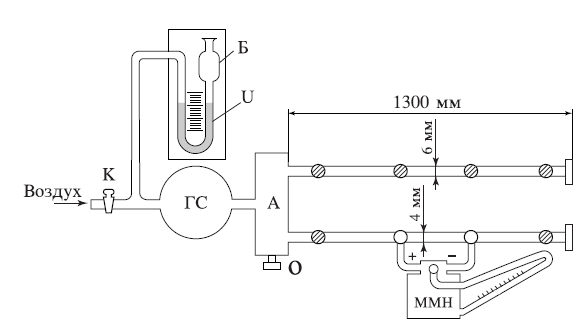
\includegraphics[width=14cm]{scheme.png}
	\end{center}
	\caption{\textit{Схема установки}}
	\label{scheme}
\end{figure}

Схема установки для исследования эффекта Джоуля–Томсона в углекислом газе представлена на рисунке \ref{scheme}. Основным элементом установки является трубка 1 с пористой перегородкой 2, через которую пропускается исследуемый газ. Трубка имеет длину 80 мм и сделана из нержавеющей стали, обладающей, как известно, малой теплопроводностью. Диаметр трубки $ d = 3 $~мм, толщина стенок 0,2 мм. Пористая перегородка расположена в конце трубки и представляет собой стеклянную пористую пробку со множеством узких и длинных каналов. Пористость и толщина пробки ($ l = 5 $ мм) подобраны так, чтобы обеспечить оптимальный поток газа при перепаде давлений $ \Delta P \leqslant 4 $ атм (расход газа составляет около $ 10 $ см$ ^3 $/с); при этом в результате эффекта Джоуля–Томсона создается достаточная разность температур.

Углекислый газ под повышенным давлением поступает в трубку через змеевик 5 из балластного баллона 6. Медный змеевик омывается водой и нагревает медленно протекающий через него газ до температуры воды в термостате. Температура воды измеряется термометром $ T_\text{в} $, помещенным в термостате. Требуемая температура воды устанавливается и поддерживается во время эксперимента при помощи контактного термометра $ T_\text{к} $.

Давление газа в трубке измеряется манометром М и регулируется вентилем В (при открывании вентиля В, т. е. при повороте ручки против часовой стрелки, давление $ P_1 $ повышается). Манометр М измеряет разность между давлением внутри трубки и наружным (атмосферным) давлением. Так как углекислый газ после пористой перегородки выходит в область с атмосферным давлением $ P_2 $, то этот манометр непосредственно измеряет перепад давления на входе и на выходе трубки $ \Delta P = P_1 - P_2 $.

Разность температур газа до перегородки и после нее измеряется дифференциальной термопарой медь -- константан. Константановая проволока диаметром 0,1 мм соединяет спаи 8 и 9, а медные проволоки (того же диаметра) подсоединены к цифровому вольтметру 7. Отвод тепла через проволоку столь малого сечения пренебрежимо мал. Для уменьшения теплоотвода трубка с пористой перегородкой помещена в трубу Дьюара 3, стенки которой посеребрены, для уменьшения теплоотдачи, связанной с излучением. Для уменьшения теплоотдачи за счет конвекции один конец трубы Дьюара уплотнен кольцом 4, а другой закрыт пробкой 10 из пенопласта. Такая пробка практически не создает перепада давлений между внутренней полостью трубы и атмосферой.

\subsection*{Ход работы}
Проведя измерения, занесем точки в таблицу \ref{dta}. Построим графики полученных зависимостей (см. рис. \ref{fig:pot}). Из графиков заключаем - зависимость с достаточной точностью можно считать линейной. 
\begin{table}
	
	\caption{Данные}
	\label{dta}
	\centering
	\footnotesize
	\begin{tabular}{|c|c|c|c|c|c|c|c|c|}
		\hline
		\multicolumn{3}{|c|}{$20^\circ C$} & \multicolumn{3}{|c|}{$30^\circ C$} & \multicolumn{3}{|c|}{$40^\circ C$} \\ \hline
		$\Delta P$, Па & $V,$ мкВ & $\Delta T,$К & $\Delta P$, Па & $V,$ мкВ & $\Delta T,$К & $\Delta P$, Па & $V,$ мкВ & $\Delta T,$К \\ \hline
		4.00 & 130 & 3.19 & 4.00 & 125 & 3.00 & 4.00 & 115 & 2.76 \\ \hline
		3.60 & 115 & 2.83 & 3.55 & 105 & 2.52 & 3.60 & 100 & 2.40 \\ \hline
		3.20 & 97 & 2.38 & 3.15 & 88 & 2.12 & 3.15 & 84 & 2.02 \\ \hline
		2.85 & 82 & 2.01 & 2.80 & 73 & 1.75 & 2.80 & 68 & 1.63 \\ \hline
		2.40 & 60 & 1.47 & 2.45 & 58 & 1.39 & 2.45 & 56 & 1.35 \\ \hline
		2.00 & 48 & 1.18 & 2.00 & 45 & 1.08 & 2.05 & 43 & 1.03 \\ \hline
		
		\multicolumn{3}{|c|}{$45^\circ C$} & \multicolumn{3}{|c|}{$50^\circ C$} & \multicolumn{3}{|c|}{} \\ \hline
		$\Delta P$, Па & $V,$ мкВ & $\Delta T,$К & $\Delta P$, Па & $V,$ мкВ & $\Delta T,$К &  \multicolumn{3}{|c|}{} \\ \hline
		4.00 & 113 & 2.66 & 4.00 & 113 & 2.59& \multicolumn{3}{|c|}{} \\ \hline
		3.65 & 102 & 2.40 & 3.60 & 96 & 2.20& \multicolumn{3}{|c|}{} \\ \hline
		3.20 & 85 & 2.00 & 3.20 & 81 & 1.86& \multicolumn{3}{|c|}{} \\ \hline
		2.75 & 68 & 1.60 & 2.80 & 66 & 1.51& \multicolumn{3}{|c|}{} \\ \hline
		2.35 & 52 & 1.22 & 2.40 & 52 & 1.19& \multicolumn{3}{|c|}{} \\ \hline
		2.05 & 42 & 0.99 & 2.00 & 38 & 0.87& \multicolumn{3}{|c|}{} \\ \hline
		
	\end{tabular}
	
\end{table}
\begin{figure}
	\centering
	\includegraphics[width=1\linewidth]{"Температура от давления"}
	\caption{Температура от давления}
	\label{fig:pot}
\end{figure}


\begin{table}
	
	\caption{Обработка}
	\label{tab:stat}
	\centering
	\footnotesize
	\begin{tabular}{|c|c|c|c|c|c|c|c|c|c|}
		\hline
		Температура& $\overline{x}$ & $\sigma_x^2$ & $\overline{y}$ & $\sigma_y^2$ & $r_{xy}$ & $A$ & $\Delta A$ & $B$ & $\Delta B$ \\ \hline
		$20^\circ C$ & 3.008 & 0.464 & 2.179 & 0.502 & 0.482 & 1.039 & 0.028 & -0.948 & 0.087 \\ \hline
		$30^\circ C$ & 2.992 & 0.445 & 1.979 & 0.428 & 0.435 & 0.979 & 0.033 & -0.948 & 0.101 \\ \hline
		$40^\circ C$ & 3.008 & 0.438 & 1.867 & 0.356 & 0.394 & 0.901 & 0.019 & -0.844 & 0.059 \\ \hline
		$45^\circ C$ & 3.000 & 0.475 & 1.812 & 0.361 & 0.414 & 0.872 & 0.013 & -0.804 & 0.039 \\ \hline
		$50^\circ C$ & 3.000 & 0.467 & 1.705 & 0.342 & 0.399 & 0.855 & 0.015 & -0.861 & 0.046 \\ \hline
	\end{tabular}
\end{table}

\begin{figure}\CenterFloatBoxes
	\begin{floatrow}
		\ffigbox[\FBwidth]
		{\caption{Нахождение постоянных $a$ и $b$}\label{fig:pkal}}
		{
			
			\includegraphics[width=1.1\linewidth]{"Коэффициент от обратной темературы.pdf"}
			
		}
		\killfloatstyle\ttabbox[\Xhsize]
		{\caption{} \label{tab:pkal}}
		{	\footnotesize
			
			\begin{tabular}{|c|c|}
				\hline
				$T^{-1}, K^{-1}$ & $\mu, \frac{K}{\text{атм}}$ \\ \hline
				0.003411 & 1.039176 \\ \hline
				0.003299 & 0.978513 \\ \hline
				0.003193 & 0.900994 \\ \hline
				0.003143 & 0.871827 \\ \hline
				0.003095 & 0.855177 \\ \hline
			\end{tabular}
			
		}
	\end{floatrow}
\end{figure}
Перейдем к расчету зависимостей. Обработку проведем методом наименьших квадратов:

$$y = Ax + B,$$

где $$A = \frac{r_{xy}}{ \sigma_x^2},$$
$$B = \overline{y} - A\overline{x}.$$

Для оценки погрешностей используем следующие формулы:
$$\Delta A =  t_{n-1, p} \sqrt{\frac{1}{n-2} \left( \frac{\sigma_y^2}{\sigma_x^2} - A^2 \right)},$$
$$\Delta B = \Delta A \sqrt{\sigma_x^2 + \overline{x}^2},$$

где 
$n$ - количество измерений, $ t_{n-1, p}$ - коэффициент Стьюдента

\begin{table}
	
	\caption{Обработка для $\mu \left(\frac{1}{T}\right)$}
	\label{tab:ab}
	\centering
	\footnotesize
	\begin{tabular}{|c|c|c|c|c|c|c|c|c|c|}
		\hline
		$\overline{x}$ & $\sigma_x^2$ & $\overline{y}$ & $\sigma_y^2$ & $r_{xy}$ & $A$ & $\Delta A$ & $B$ & $\Delta B$ \\ \hline
		0.003 & 1.30e-08 & 0.929 & 4.82e-03 & 0.000 & 607.622 & 3.020e+01 & -1.032 & 0.098 \\ \hline
	\end{tabular}
\end{table}
По угловому коэффициенту получаем значения $\mu_\text{Д--Т} = \frac{\Delta T}{\Delta P} = A$.

Для нахождения коэффициентов $a$ и $b$ газа, перепишем зависимость \ref{3} в виде:

\begin{equation}\label{5}
	\mu_\text{Д--Т} = \frac{2a}{C_P T} - \frac{b}{C_P}.
\end{equation}

Для приведенной выше зависимости \ref{5} легко провести линеаризацию, рассмотрев $\mu_\text{Д--Т}\left(\frac{1}{T}\right)$. Пересчет занесем в таблицу \ref{tab:pkal}. Построим график, чтобы убедится, что зависимость вообще можно считать линейной. Проведем обработку методом наименьших квадратов (см. таблицу \ref{tab:ab}), откуда получаем

\begin{equation}
	\mu_\text{Д--Т} = A\frac{1}{T} + B,
\end{equation}

где $$A = \frac{2a}{C_P T} = (61 \pm 3)\e{2} \text{  }\text{атм}^{-1}, $$
	$$B = - \frac{b}{C_P} = (-1.0 \pm 0.1) \text{  }K\cdot \text{атм}^{-1}.$$

Проведем расчет коэффициентов $a$ и $b$:
$$a = (1.01 \pm 0.06) \frac{H\cdot\text{м}^2}{\text{моль}^2}$$

$$b = (41 \pm 4)\e{1} \frac{\text{см}^3}{\text{моль}}$$

Для критической температуры получаем:
$$T_\text{кр} = \frac{8a}{27Rb} \approx 90 \text{ К}$$













\subsection*{Вывод}

Несмотря на достаточно маленькие погрешности видно, что значения коэффициентов сильно отличаются от табличных $a_\text{таб.} = 0.36\frac{H\cdot\text{м}^2}{\text{моль}^2}$ и $b_\text{таб.}= 42.2\frac{\text{см}^3}{\text{моль}}$.

Однако видно, что данная модель весьма неплохо описывает качественное поведение процесса. Графики оказались линейными, а погрешности коэффициентов зависимости малы. 
Объяснить различие можно попробовать большой систематической погрешностью. 

Для уточнения результатов стоит обратить внимание на точность измерения температуры и особенно давления.


\end{document}